% !TEX program = xelatex
% Beamer + Metropolis. Компилировать XeLaTeX (в VS Code это видит строка выше).
% Картинки берутся из ../experiments/plots/ (см. \graphicspath).
\documentclass[aspectratio=169]{beamer}
\usetheme{metropolis}

\usepackage{FiraSans}   % шрифт Metropolis с кириллицей (из TeX Live, портативно)
\usepackage{FiraMono}
\usepackage{polyglossia}
\setmainlanguage{russian}
\setotherlanguage{english}

\usepackage{booktabs}   % красивые таблицы
\usepackage{amsmath}
\usepackage{tikz}
\usetikzlibrary{positioning, arrows.meta}
\tikzset{
  vblk/.style={draw, rounded corners=2pt, align=center, font=\scriptsize,
               text width=3.6cm, minimum height=5.5mm, inner sep=3pt},
  vio/.style={vblk, fill=black!6},
  vbb/.style={vblk, fill=black!18},        % Transolver - чёрный ящик
  vop/.style={vblk, fill=blue!8},
  var/.style={-{Stealth[length=2mm]}, semithick},
}
\usepackage[absolute,overlay]{textpos}   % абсолютное позиционирование (сноски у низа)
\textblockorigin{0pt}{0pt}

\graphicspath{{../experiments/plots/}{res/}}

% автогенерация gen_metrics.py из experiments/*/metrics.json -- руками не править
\newcommand{\mTrivialNskMean}{22.4}
\newcommand{\mTrivialNskSmooth}{29.8}
\newcommand{\mTrivialSakMean}{6.6}
\newcommand{\mTrivialSakSmooth}{7.9}
\newcommand{\mPhysMean}{20.5}
\newcommand{\mPhysSmooth}{17.5}
\newcommand{\mFieldMean}{16.2}
\newcommand{\mFieldSmooth}{21.0}
\newcommand{\mHeatMean}{3.6}
\newcommand{\mHeatSmooth}{2.1}
\newcommand{\mRegMean}{20.3}
\newcommand{\mRegSmooth}{20.3}
\newcommand{\mUnetMean}{1.6}
\newcommand{\mUnetSmooth}{1.5}
\newcommand{\mWindNoMean}{2.6}
\newcommand{\mWindNoSmooth}{2.5}
\newcommand{\mWindYesMean}{5.0}
\newcommand{\mWindYesSmooth}{2.0}
\newcommand{\mPinnMean}{2.6}
\newcommand{\mPinnSmooth}{1.6}
   % макросы метрик, генерит gen_metrics.py из experiments/*/metrics.json

\title{Исследование загрязнений с помощью предсказаний локальной погоды}
% \subtitle{Сравнение подходов: Transolver, UNet, PINN}
\author{Чертан Вячеслав Александрович}
\institute{ИИ360 НИУ ВШЭ}
\date{\today}

\begin{document}

% --- титул ---
\maketitle

% --- слайд "Введение" (3 иконки, как в зимней презе) ---
\begin{frame}[t]{Введение}
  \vskip0pt plus1filll
  % \vspace{1em}
  \begin{columns}[t,onlytextwidth]
    \begin{column}{0.30\textwidth}
      \centering
      \includegraphics[height=2.3cm]{cough.pdf}\\[0.9em]
      {\LARGE\textbf{4.2 млн}}\\[0.6em]
      {\fontsize{6pt}{7.5pt}\selectfont Преждевременных смертей из-за загрязнения воздуха за год\textsuperscript{*}\par}

    \end{column}\hfill
    \begin{column}{0.30\textwidth}
      \centering
      \includegraphics[height=2.3cm]{dust.pdf}\\[0.9em]
      {\LARGE\textbf{5 мкг\,/\,м\textsuperscript{3}}}\\[0.6em]
      {\fontsize{6pt}{7.5pt}\selectfont Среднегодовая норма содержания PM2.5\textsuperscript{**}\par}
    \end{column}\hfill
    \begin{column}{0.30\textwidth}
      \centering
      \includegraphics[height=2.3cm]{computer.pdf}\\[0.9em]
      {\LARGE\textbf{Симуляция}}\\[0.6em]
      {\fontsize{6pt}{7.5pt}\selectfont Слишком медленное решение для оперативного реагирования\par}
    \end{column}
  \end{columns}
  \vskip0pt plus1filll
  \begin{textblock*}{0.92\paperwidth}(0.04\paperwidth, 0.87\paperheight)
    {\fontsize{6pt}{6.5pt}\selectfont
      \textsuperscript{*}~по данным ВОЗ: \textenglish{\url{https://www.who.int/news-room/fact-sheets/detail/ambient-(outdoor)-air-quality-and-health}}\\[1pt]
      \textsuperscript{**}~по данным ВОЗ: \textenglish{\url{https://www.who.int/teams/environment-climate-change-and-health/air-quality-and-health/health-impacts/types-of-pollutants}}\par}
  \end{textblock*}
\end{frame}

% --- слайд "Постановка задачи" ---
\begin{frame}{Постановка задачи}
  \textbf{Цель:} по динамике концентрации PM2.5 (и полю ветра, где оно есть)
  определить координаты источника выброса

  \vspace{0.4em}
  \begin{center}
    \begin{tabular}{lcc}
      \toprule
                         & \textbf{Новосибирск} & \textbf{Сахалин} \\
      \midrule
      Сетка              & $251 \times 201$ & $300 \times 300$ \\
      Ветер (U10, V10)   & нет              & есть \\
      Файлов             & 49               & 15 \\
      Уникальных источников & 10               & 19 \\
      \bottomrule
    \end{tabular}
  \end{center}

  \vspace{0.4em}
  \textbf{Вход:} 17 кадров ($t = 1..17$)\\
  \textbf{Метка:} $(x, y)$ координаты выброса\\
  \textbf{Метрика:} евклидова ошибка локализации в клетках
\end{frame}

\begin{frame}{Подходы к локализации}
  \begin{itemize}
    \item Тривиальный бейзлайн
    \item Физический бейзлайн
    \item Transolver
    \item Transolver + heatmap
    \item Transolver + regression
    \item UNet + heatmap
    \item Transolver + heatmap + ветер
    \item PINN
  \end{itemize}
\end{frame}

\begin{frame}{Функция потерь}
  \textbf{Loss} = взвешенная сумма:
  \begin{itemize}
    \item \textbf{field} --- реконструкция поля $C_{t=0}$
    \item \textbf{heatmap} --- spatial softmax, карта вероятности источника
    \item \textbf{coord} --- регрессия $(x, y)$
  \end{itemize}

  \[
    \mathcal{L} = w_f\,\mathcal{L}_{\text{field}} + w_h\,\mathcal{L}_{\text{heat}}
                + w_c\,\mathcal{L}_{\text{coord}} + w_p\,\mathcal{L}_{\text{PDE}}
  \]
  \vspace{-0.4em}
  \[
    \mathcal{L}_{\text{field}}=\frac{\lVert\hat C-C\rVert_2}{\lVert C\rVert_2},\quad
    \mathcal{L}_{\text{heat}}=\mathrm{KL}(p_{\text{true}}\,\Vert\,p_{\text{pred}}),\quad
    \mathcal{L}_{\text{coord}}=\lVert\hat{x}-x\rVert_2^2
  \]
\end{frame}

\section{Бейзлайны}

\begin{frame}{Тривиальный бейзлайн --- архитектура}
  \begin{columns}[T,onlytextwidth]
    \begin{column}{0.5\textwidth}
      \vspace{0.6em}
      \textbf{Ошибка на тесте:}
      \begin{itemize}
        \item без сглаживания --- \textbf{\mTrivialNskMean}
        \item со сглаживанием --- \textbf{\mTrivialNskSmooth}
      \end{itemize}
    \end{column}
    \begin{column}{0.45\textwidth}
      \centering
      \begin{tikzpicture}[node distance=2.4mm]
        \node[vio](a){$C_{t=17}$};
        \node[vop, below=of a](b){$\arg\max$};
        \node[vio, below=of b](c){source};
        \draw[var](a)--(b); \draw[var](b)--(c);
      \end{tikzpicture}
    \end{column}
  \end{columns}
\end{frame}

\begin{frame}{Тривиальный бейзлайн --- примеры}
  \vspace{0.4em}
  \centering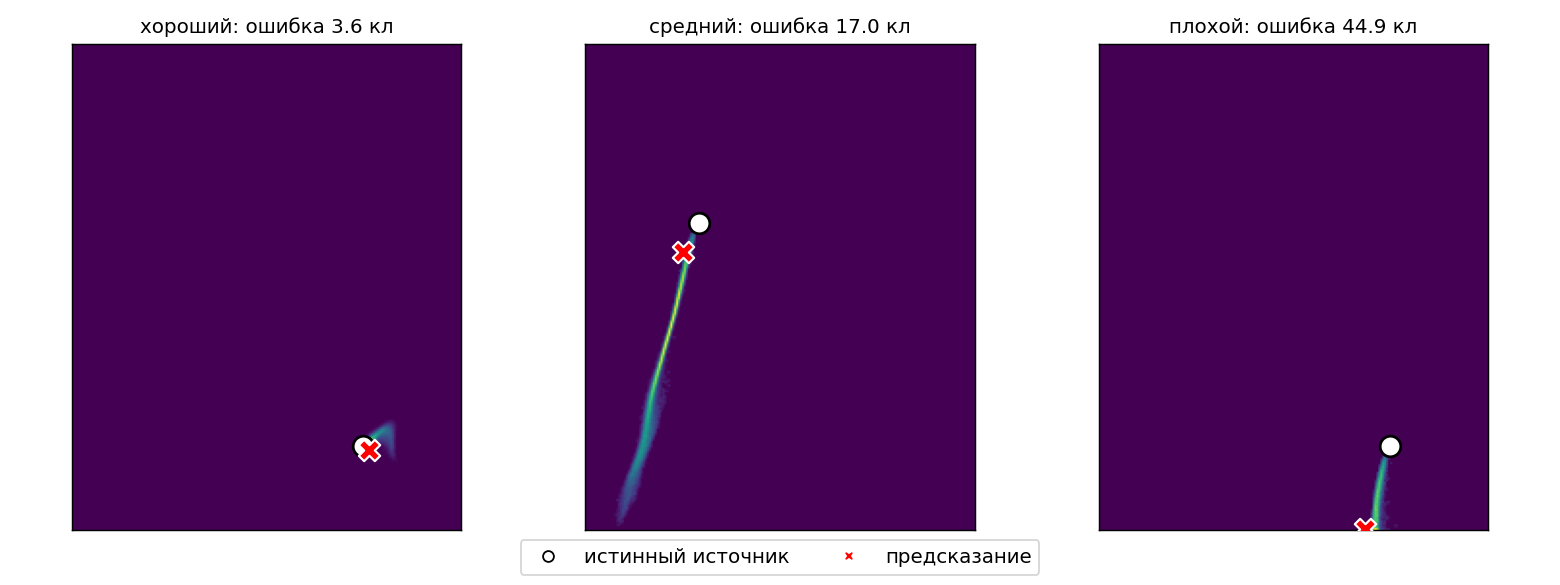
\includegraphics[width=1\textwidth]{demo_trivial.png}
\end{frame}

\begin{frame}{Физический бейзлайн --- архитектура}
  \begin{columns}[T,onlytextwidth]
    \begin{column}{0.5\textwidth}
      % \textbf{Функция потерь:} нет --- численный метод (нужен ветер $\Rightarrow$ Сахалин).

      \vspace{0.6em}
      \textbf{Ошибка на тесте:}
      \begin{itemize}
        \item без сглаживания --- \textbf{\mPhysMean}
        \item со сглаживанием --- \textbf{\mPhysSmooth}
      \end{itemize}
    \end{column}
    \begin{column}{0.45\textwidth}
      \centering
      \begin{tikzpicture}[node distance=2.4mm]
        \node[vio](a){$C_{t=1}, (U, V)_{t=1}$};
        \node[vop, below=of a](b){обратная адвекция};
        \node[vio, below=of b](c){source = $\arg\max$};
        \draw[var](a)--(b); \draw[var](b)--(c);
      \end{tikzpicture}
    \end{column}
  \end{columns}
\end{frame}

\begin{frame}{Физический бейзлайн --- примеры}
  \vspace{0.4em}
  \centering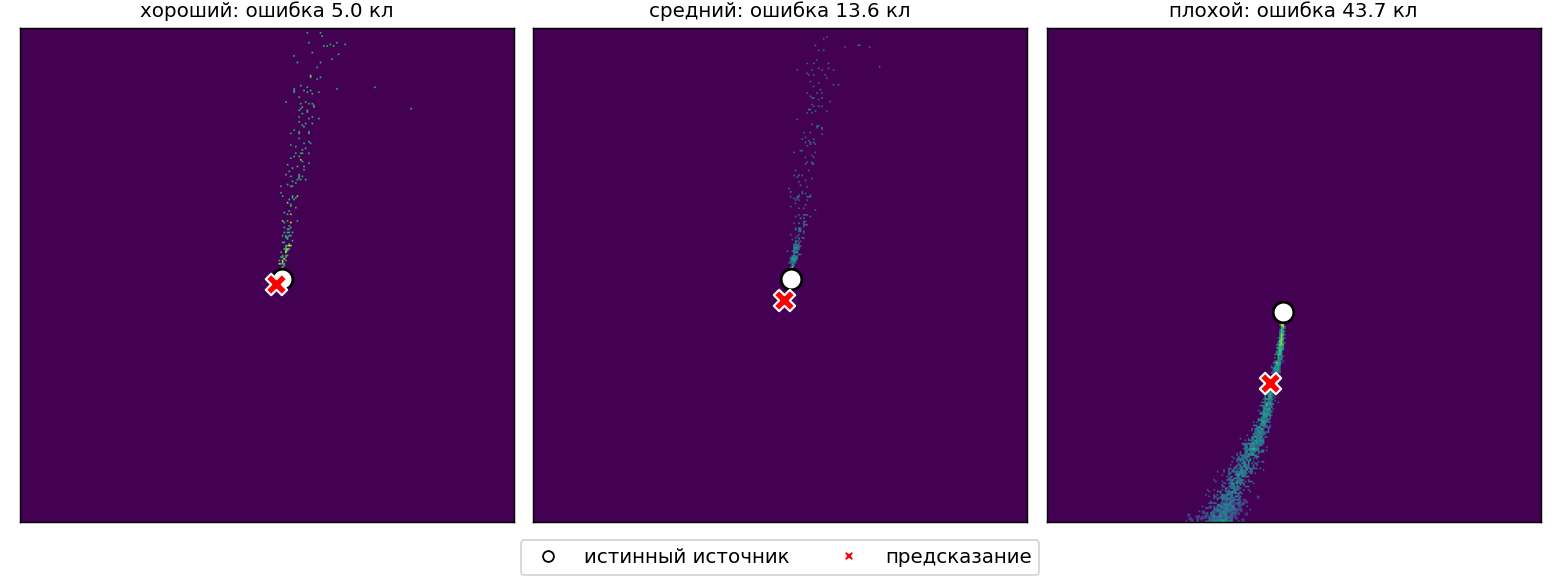
\includegraphics[width=1\textwidth]{demo_physical.png}
\end{frame}

\section{Обучаемые модели}

\begin{frame}{Transolver (только поле) --- архитектура}
  \begin{columns}[T,onlytextwidth]
    \begin{column}{0.5\textwidth}
      \textbf{Функция потерь:}
      \[ \mathcal{L} = \mathcal{L}_{\text{field}} \]

      \vspace{0.6em}
      \textbf{Ошибка на тесте:}
      \begin{itemize}
        \item без сглаживания --- \textbf{\mFieldMean}
        \item со сглаживанием --- \textbf{\mFieldSmooth}
      \end{itemize}
    \end{column}
    \begin{column}{0.45\textwidth}
      \centering
      \begin{tikzpicture}[node distance=2.4mm]
        \node[vio](a){$[C_{t=1}, \dots, C_{t=17}]$ \ ($17{\times}H{\times}W$)};
        \node[vbb, below=of a](b){Transolver $\to$ $C_{t=0}$};
        \node[vio, below=of b](c){source $=\arg\max$};
        \draw[var](a)--(b); \draw[var](b)--(c);
      \end{tikzpicture}
    \end{column}
  \end{columns}
\end{frame}

\begin{frame}{Transolver (только поле) --- примеры}
  \vspace{0.4em}
  \centering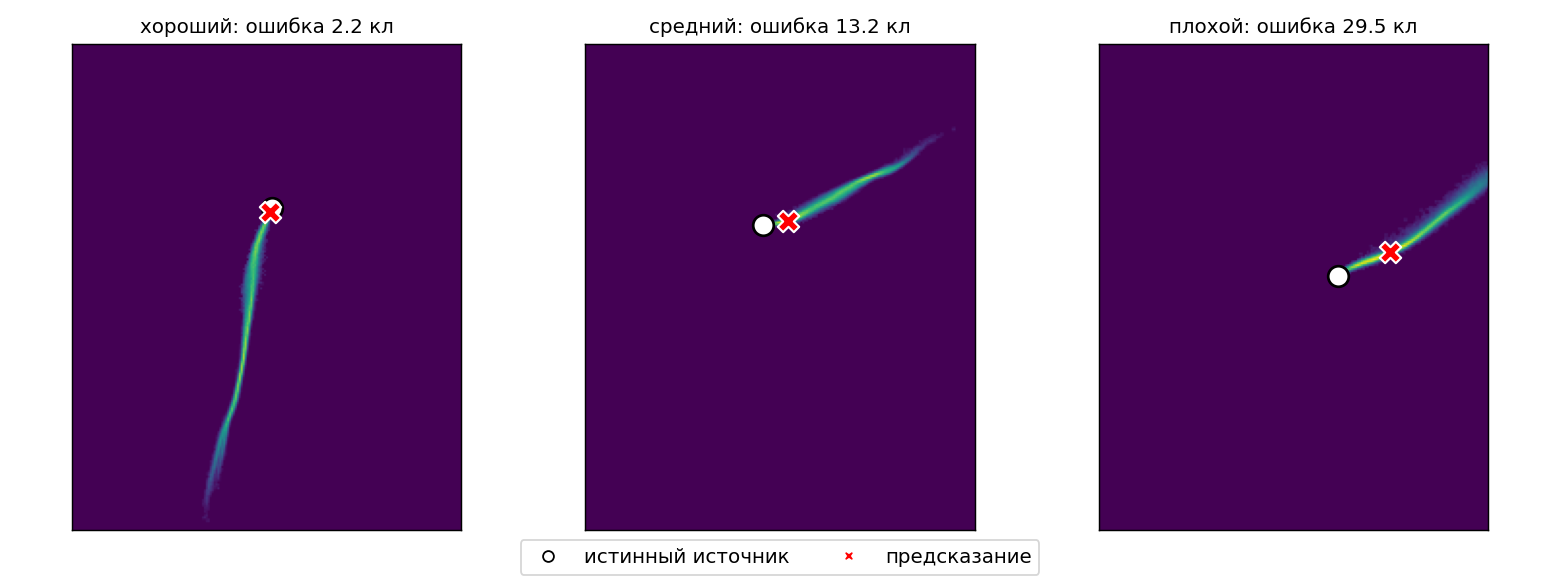
\includegraphics[width=1\textwidth]{demo_field_only.png}
\end{frame}

\begin{frame}{Transolver + heatmap --- архитектура}
  \begin{columns}[T,onlytextwidth]
    \begin{column}{0.5\textwidth}
      \textbf{Функция потерь:}
      \[ \mathcal{L} = \mathcal{L}_{\text{field}} + \mathcal{L}_{\text{heat}} \]

      \vspace{0.6em}
      \textbf{Ошибка на тесте:}
      \begin{itemize}
        \item без сглаживания --- \textbf{\mHeatMean}
        \item со сглаживанием --- \textbf{\mHeatSmooth} 
      \end{itemize}
    \end{column}
    \begin{column}{0.45\textwidth}
      \centering
      \begin{tikzpicture}[node distance=2.4mm]
        \node[vio](a){$[C_{t=1}, \dots, C_{t=17}]$ \ ($17{\times}H{\times}W$)};
        \node[vbb, below=of a](b){Transolver $\to$ $C_{t=0}$};
        \node[vop, below=of b](c){Conv $3{\times}3$,\ $1\!\to\!64$,\ GELU};
        \node[vop, below=of c](d){Conv $3{\times}3$,\ $64\!\to\!64$,\ GELU\ ($\times2$)};
        \node[vop, below=of d](e){Conv $1{\times}1$,\ $64\!\to\!1$};
        \node[vop, below=of e](f){spatial softmax};
        \node[vio, below=of f](g){source $=\arg\max$};
        \draw[var](a)--(b); \draw[var](b)--(c); \draw[var](c)--(d);
        \draw[var](d)--(e); \draw[var](e)--(f); \draw[var](f)--(g);
      \end{tikzpicture}
    \end{column}
  \end{columns}
\end{frame}

\begin{frame}{Transolver + heatmap --- примеры}
  \vspace{0.4em}
  \centering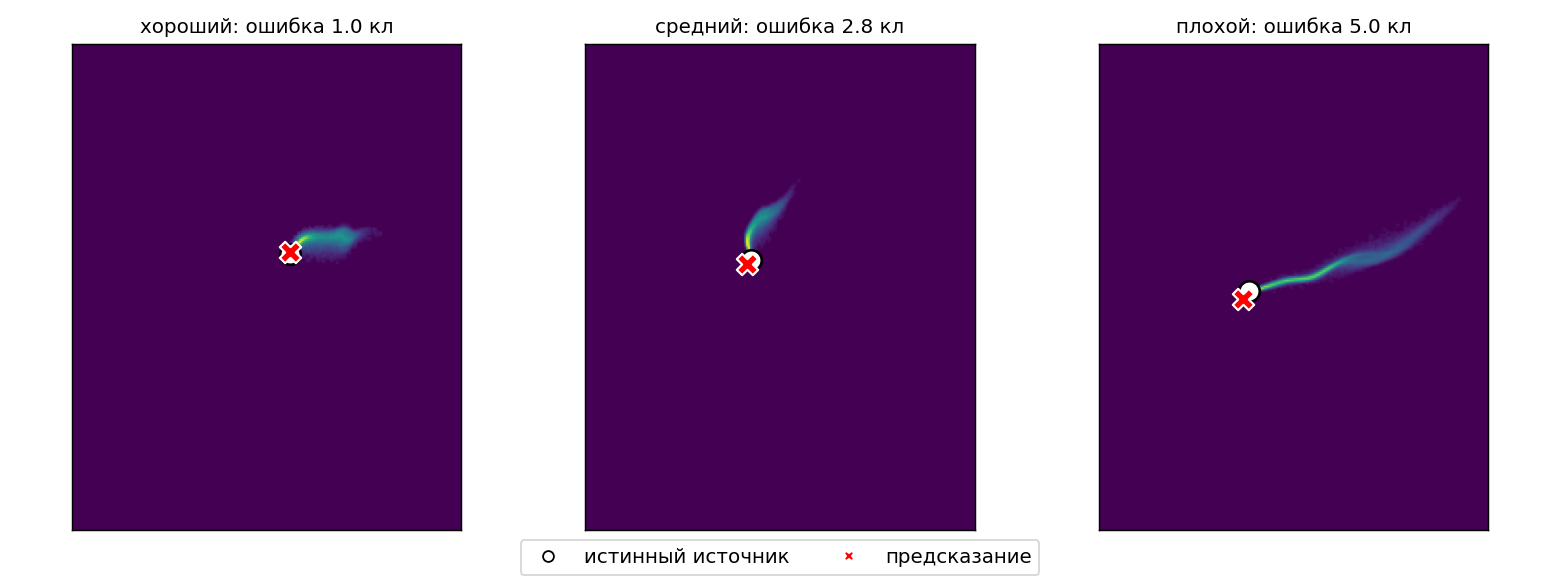
\includegraphics[width=1\textwidth]{demo_heatmap.png}
\end{frame}

\begin{frame}{Transolver + regression --- архитектура}
  \begin{columns}[T,onlytextwidth]
    \begin{column}{0.5\textwidth}
      \textbf{Функция потерь:}
      \[ \mathcal{L} = \mathcal{L}_{\text{field}} + 0.001\,\mathcal{L}_{\text{coord}} \]

      \vspace{0.6em}
      \textbf{Ошибка на тесте: \mRegMean}
    \end{column}
    \begin{column}{0.45\textwidth}
      \centering
      \begin{tikzpicture}[node distance=2.4mm]
        \node[vio](a){$[C_{t=1}, \dots, C_{t=17}]$ \ ($17{\times}H{\times}W$)};
        \node[vbb, below=of a](b){Transolver $\to$ $C_{t=0}$};
        \node[vop, below=of b](c){Conv $3{\times}3$,\ $1\!\to\!64$,\ GELU};
        \node[vop, below=of c](d){Conv $3{\times}3$,\ $64\!\to\!64$,\ GELU\ ($\times2$)};
        \node[vop, below=of d](e){AvgPool $8$ $\to$ Linear $128$ $\to$ Linear $2$};
        \node[vio, below=of e](f){source $=(x,y)$};
        \draw[var](a)--(b); \draw[var](b)--(c); \draw[var](c)--(d);
        \draw[var](d)--(e); \draw[var](e)--(f);
      \end{tikzpicture}
    \end{column}
  \end{columns}
\end{frame}

\begin{frame}{Transolver + regression --- примеры}
  \vspace{0.4em}
  \centering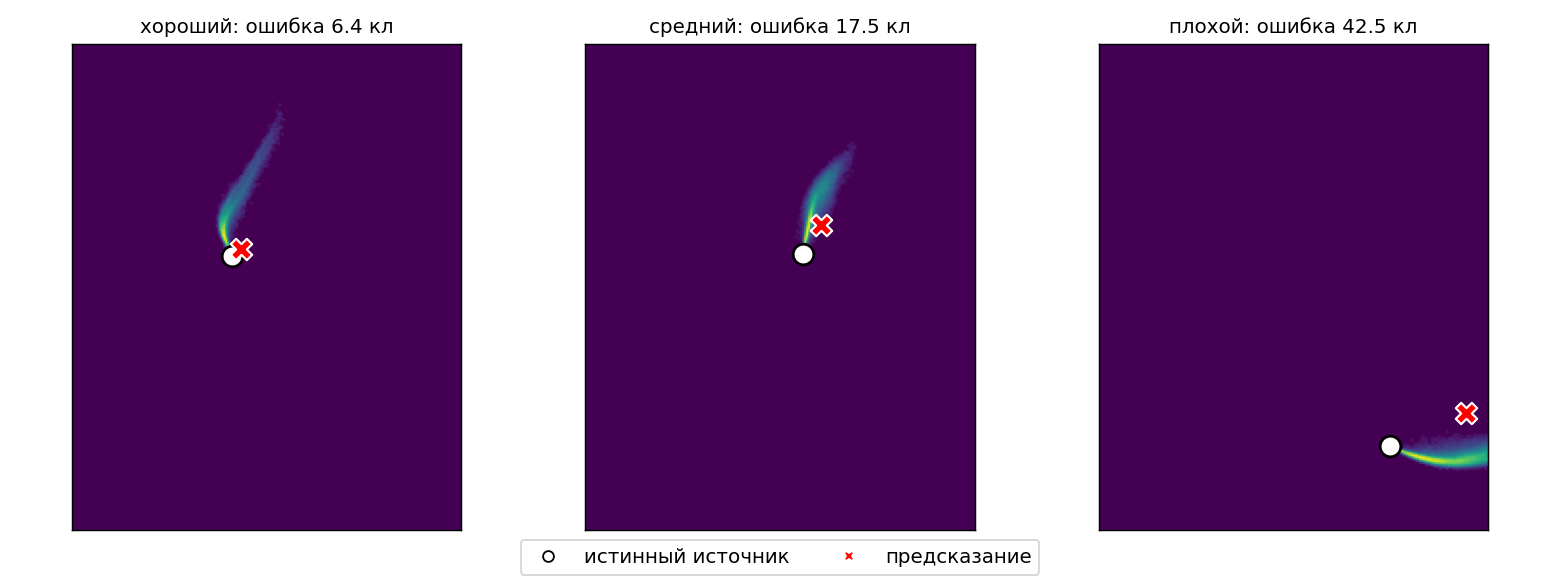
\includegraphics[width=1\textwidth]{demo_regressor.png}
\end{frame}

\begin{frame}{UNet + heatmap --- архитектура}
  \begin{columns}[T,onlytextwidth]
    \begin{column}{0.5\textwidth}
      \textbf{Функция потерь:}
      \[ \mathcal{L} = \mathcal{L}_{\text{field}} + \mathcal{L}_{\text{heat}} \]

      \vspace{0.6em}
      \textbf{Ошибка на тесте:}
      \begin{itemize}
        \item без сглаживания --- \textbf{\mUnetMean}
        \item со сглаживанием --- \textbf{\mUnetSmooth}
      \end{itemize}
    \end{column}
    \begin{column}{0.45\textwidth}
      \centering
      \begin{tikzpicture}[node distance=2.4mm]
        \node[vio](a){$[C_{t=1}, \dots, C_{t=17}]$ \ ($17{\times}H{\times}W$)};
        \node[vop, below=of a](b){Энкодер $32\!\to\!64\!\to\!128$\\(Conv+GN+GELU, pool)};
        \node[vop, below=of b](c){Bottleneck $256$};
        \node[vop, below=of c](d){Декодер $128\!\to\!64\!\to\!32$\\(upconv $+$ skip)};
        \node[vop, below=of d](e){Conv $1{\times}1$ $\to$ heatmap};
        \node[vio, below=of e](f){source $=\arg\max$};
        \draw[var](a)--(b); \draw[var](b)--(c); \draw[var](c)--(d);
        \draw[var](d)--(e); \draw[var](e)--(f);
      \end{tikzpicture}
    \end{column}
  \end{columns}
\end{frame}

\begin{frame}{UNet + heatmap --- примеры}
  \vspace{0.4em}
  \centering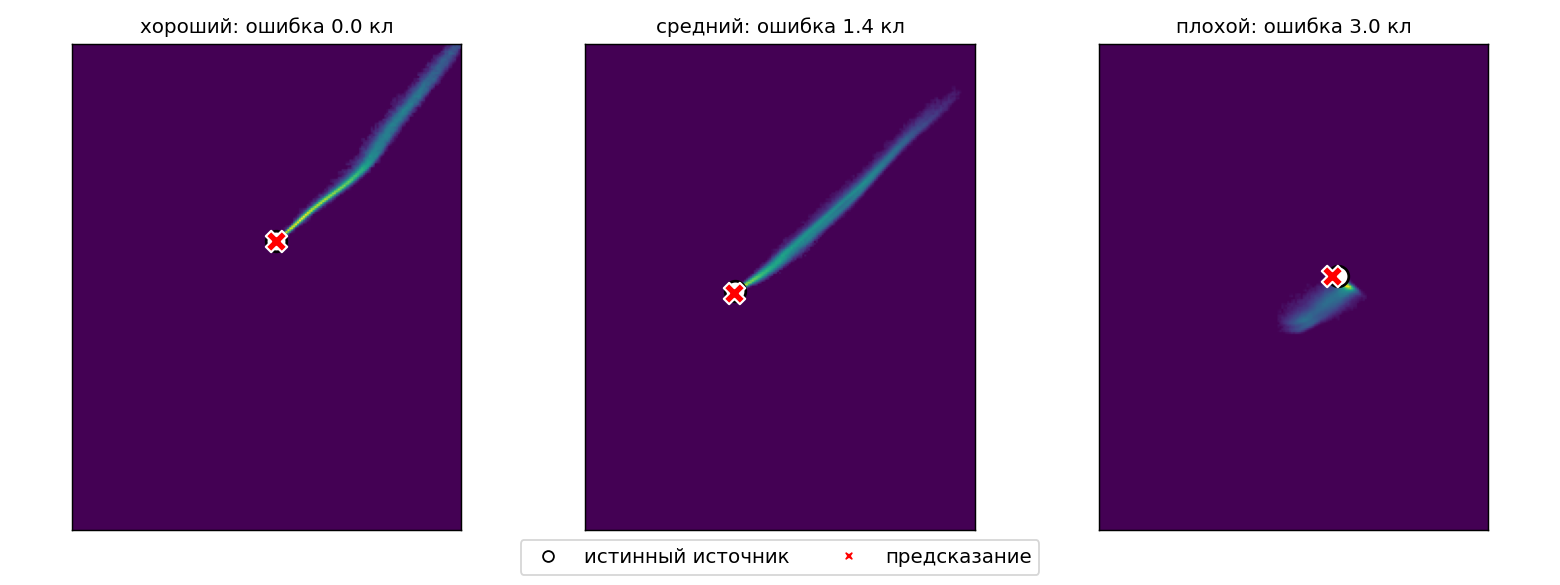
\includegraphics[width=1\textwidth]{demo_unet.png}
\end{frame}

\begin{frame}{Transolver + heatmap + ветер --- архитектура}
  \begin{columns}[T,onlytextwidth]
    \begin{column}{0.5\textwidth}
      \textbf{Функция потерь:}
      \[ \mathcal{L} = \mathcal{L}_{\text{field}} + \mathcal{L}_{\text{heat}} \]

      \vspace{0.6em}
      \textbf{Ошибка на тесте:}
      \begin{itemize}
        \item без сглаживания --- без ветра \textbf{\mWindNoMean}, с ветром \textbf{\mWindYesMean}
        \item со сглаживанием --- без ветра \textbf{\mWindNoSmooth}, с ветром \textbf{\mWindYesSmooth}
      \end{itemize}

      {\footnotesize Разброс между прогонами велик ($n{=}57$): по среднему различие в пределах шума, со сглаживанием ветер чуть лучше.\par}
    \end{column}
    \begin{column}{0.45\textwidth}
      \centering
      \begin{tikzpicture}[node distance=2.4mm]
        \node[vio](a){$C_{t=1, \ldots, 17} + (U, V)_{t=1, \ldots, 17}$ \ ($51{\times}H{\times}W$)};
        \node[vbb, below=of a](b){Transolver $\to$ $C_{t=0}$};
        \node[vop, below=of b](c){Conv $3{\times}3$,\ $1\!\to\!64$,\ GELU};
        \node[vop, below=of c](d){Conv $3{\times}3$,\ $64\!\to\!64$,\ GELU\ ($\times2$)};
        \node[vop, below=of d](e){Conv $1{\times}1$,\ $64\!\to\!1$};
        \node[vop, below=of e](f){spatial softmax};
        \node[vio, below=of f](g){source $=\arg\max$};
        \draw[var](a)--(b); \draw[var](b)--(c); \draw[var](c)--(d);
        \draw[var](d)--(e); \draw[var](e)--(f); \draw[var](f)--(g);
      \end{tikzpicture}
    \end{column}
  \end{columns}
\end{frame}

\begin{frame}{Transolver + heatmap + ветер --- примеры}
  \vspace{0.4em}
  \centering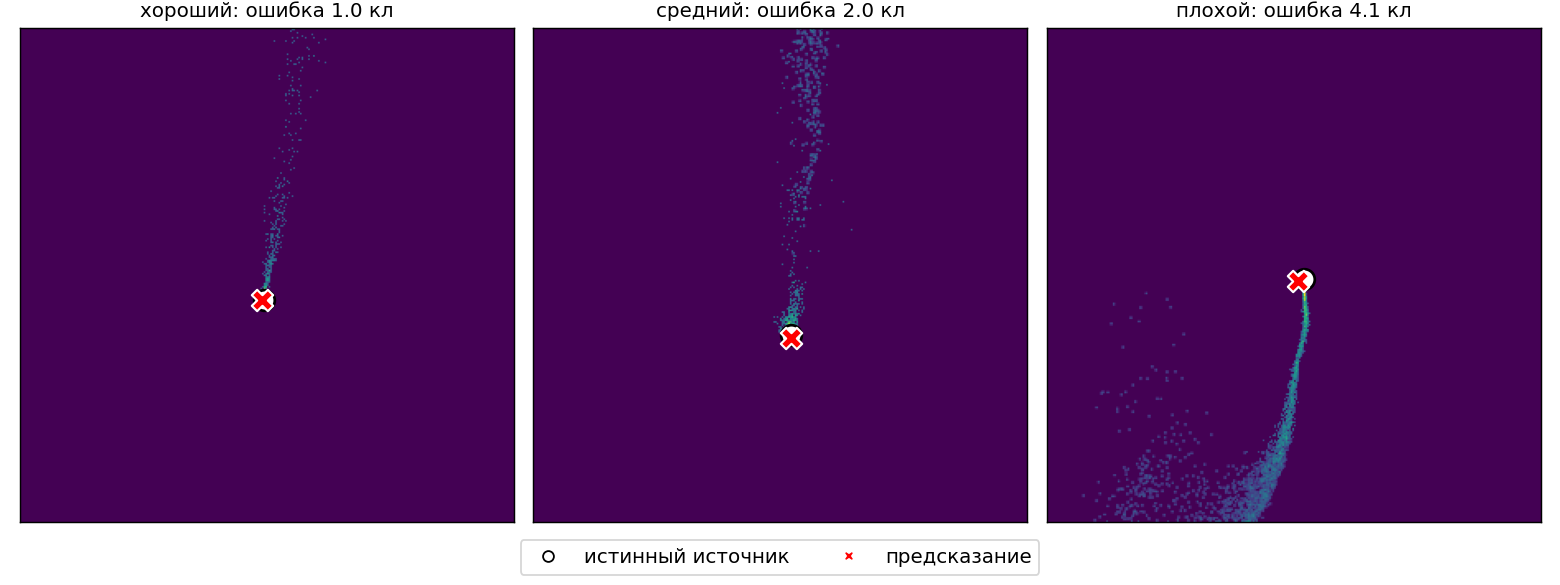
\includegraphics[width=1\textwidth]{demo_wind.png}
\end{frame}

\begin{frame}{PINN --- архитектура}
  \begin{columns}[T,onlytextwidth]
    \begin{column}{0.5\textwidth}
      \textbf{Функция потерь:}
      \[ \mathcal{L} = \mathcal{L}_{\text{field}} + \mathcal{L}_{\text{heat}} + 0.1\,\mathcal{L}_{\text{PDE}} \]

      \vspace{0.6em}
      \textbf{Ошибка на тесте:}
      \begin{itemize}
        \item без сглаживания --- \textbf{\mPinnMean}
        \item со сглаживанием --- \textbf{\mPinnSmooth}
      \end{itemize}
    \end{column}
    \begin{column}{0.45\textwidth}
      \centering
      \begin{tikzpicture}[node distance=2.4mm]
        \node[vio](a){$[C_{t=1}, \dots, C_{t=17}]$ \ ($17{\times}H{\times}W$)};
        \node[vop, below=of a](b){Conv $3{\times}3$,\ $17\!\to\!64$,\ GELU};
        \node[vop, below=of b](c){Conv $3{\times}3$,\ $64\!\to\!64$,\ GELU\ ($\times3$)};
        \node[vop, below=of c](d){Conv $1{\times}1$ $\to$ field, heatmap};
        \node[vio, below=of d](e){source $=\arg\max$};
        \draw[var](a)--(b); \draw[var](b)--(c); \draw[var](c)--(d); \draw[var](d)--(e);
      \end{tikzpicture}
    \end{column}
  \end{columns}
\end{frame}

\begin{frame}{PINN --- физический лосс}
  \[ \mathcal{L}_{\text{PDE}} = \lVert R \rVert_2^2 \]
  \vspace{-0.7em}
  \[ R = \big(C_{t=1} - \hat{C}_{t=0}\big) + u \odot \partial_x \hat{C}_{t=0}
       + v \odot \partial_y \hat{C}_{t=0} - 0.1\,\nabla^2 \hat{C}_{t=0} \]

  \vspace{0.2em}
  \[ \partial_x f_{i, j} = \frac{f_{i+1,j} - f_{i-1,j}}{2}, \qquad
     \partial_y f_{i, j} = \frac{f_{i,j+1} - f_{i,j-1}}{2} \]
  \vspace{-0.6em}
  \[ \nabla^2 f_{i, j} = f_{i+1,j} + f_{i-1,j} + f_{i,j+1} + f_{i,j-1} - 4 f_{i,j} \]
\end{frame}

\begin{frame}{PINN --- примеры}
  \vspace{0.4em}
  \centering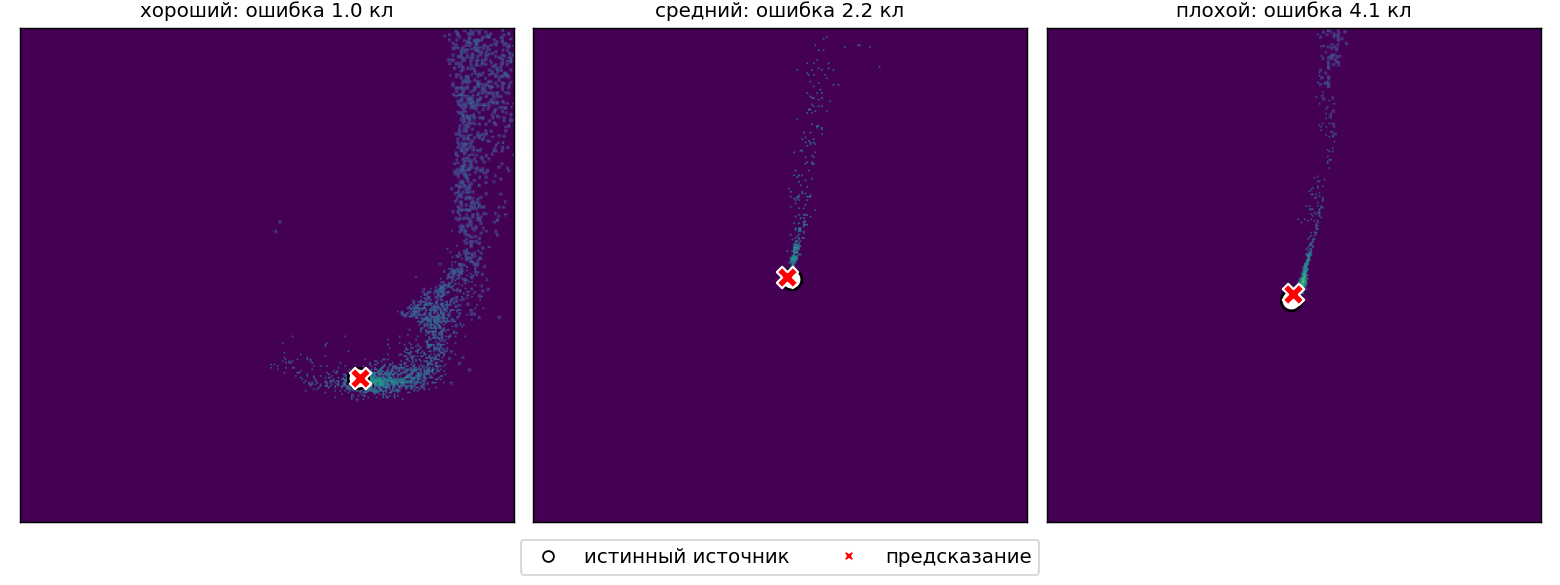
\includegraphics[width=1\textwidth]{demo_pinn.png}
\end{frame}

% --- слайд: итоговое сравнение (актуальные числа) ---
\begin{frame}{Сравнение методов --- ошибка локализации (клетки)}
  \begin{columns}[T,onlytextwidth]
    \begin{column}{0.5\textwidth}
      \centering
      \textbf{Новосибирск} ($n=100$)\\[0.3em]
      {\scriptsize
      \begin{tabular}{lcc}
        \toprule
        Метод & без сгл. & со сгл. \\
        \midrule
        UNet + heatmap         & \textbf{\mUnetMean} & \textbf{\mUnetSmooth} \\
        Transolver + heatmap   & \mHeatMean          & \mHeatSmooth \\
        Transolver (поле)      & \mFieldMean         & \mFieldSmooth \\
        Transolver + регрессия & \mRegMean           & \mRegSmooth \\
        Trivial                & \mTrivialNskMean    & \mTrivialNskSmooth \\
        \bottomrule
      \end{tabular}}
    \end{column}
    \begin{column}{0.5\textwidth}
      \centering
      \textbf{Сахалин} ($n=57$)\\[0.3em]
      {\scriptsize
      \begin{tabular}{lcc}
        \toprule
        Метод & без сгл. & со сгл. \\
        \midrule
        PINN                             & \textbf{\mPinnMean} & \textbf{\mPinnSmooth} \\
        Transolver + heatmap (без ветра) & \mWindNoMean        & \mWindNoSmooth \\
        Transolver + heatmap (ветер)     & \mWindYesMean       & \mWindYesSmooth \\
        Trivial                          & \mTrivialSakMean    & \mTrivialSakSmooth \\
        Физический                       & \mPhysMean          & \mPhysSmooth \\
        \bottomrule
      \end{tabular}}
    \end{column}
  \end{columns}

  {\scriptsize
    \begin{itemize}
      \item UNet работает лучше, чем Transolver (вероятно, из-за небольшого объема данных)
      \item Предсказывать карту вероятностей лучше, чем делать регрессию координату
      \item При наличии ветра и меньшем обьеме данных, можно получить сопоставимый с большим объемом данных результат
    \end{itemize}
  }

\end{frame}

% --- слайд с картинкой ---
\begin{frame}{Сравнение методов на тесте}
  \centering
  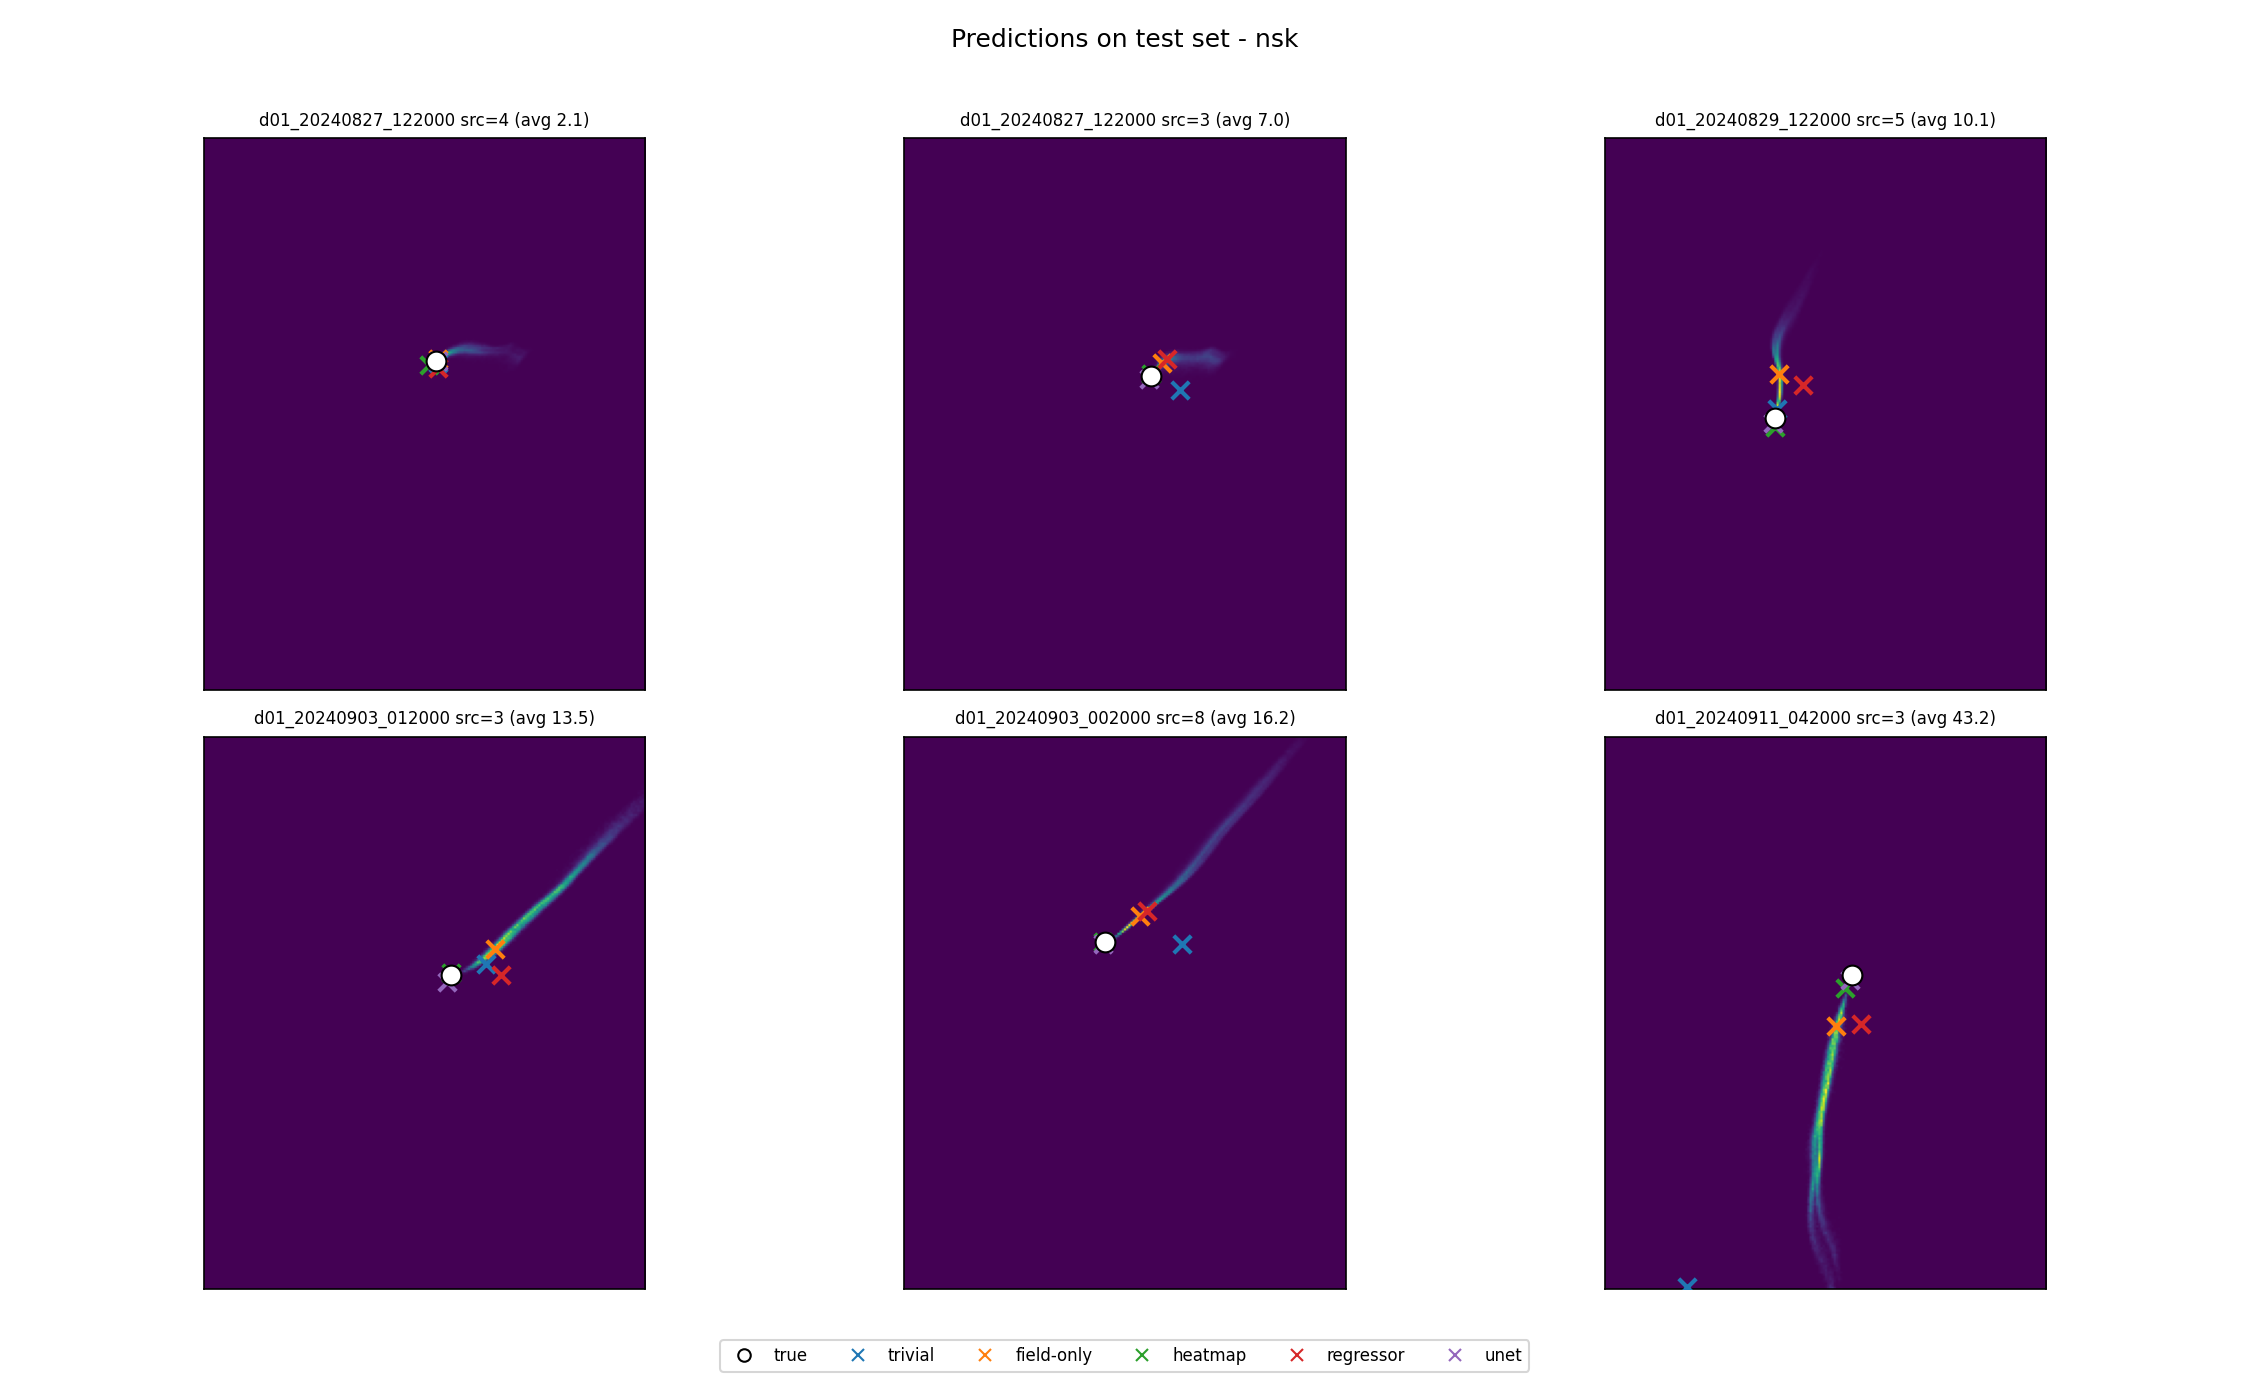
\includegraphics[width=0.9\textwidth]{compare_nsk.png}
\end{frame}

\end{document}
